\section{Vorbereitung}
\textbf{Die Versuchsvorbereitung ist Bestandteil des Versuchs. Sie erhalten dafür ein gesondertes Testat.\\\ \\
Ohne testierte Vorbereitung können Sie den Versuch nicht durchführen.  }
\begin{enumerate}[label=\alph*)]
  \item Für die Versuchsdurchführung verwenden Sie das im Labortisch eingebaute Netzmodell nach Bild ~\ref{img2.1.1}. Skizzieren Sie eine Schaltung zur Bestimmung der Netzform (siehe Aufgabe 3.1) 
    \begin{figure}[h!]
      \begin{center}
        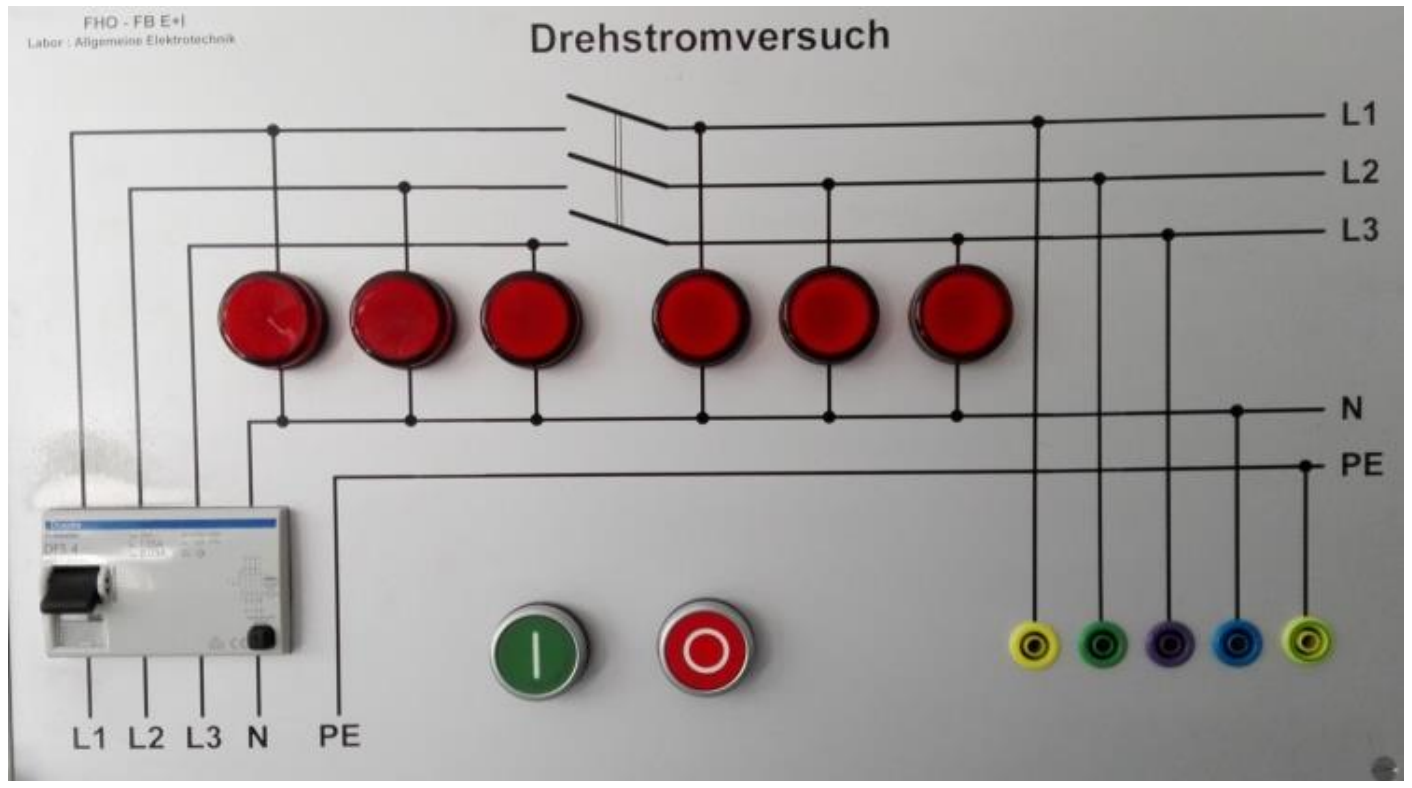
\includegraphics[width=0.5\textwidth]{img/img2.1.1.png}
      \end{center}
      \caption{Netzmodell am Versuchstisch }\label{img2.1.1}
    \end{figure}
    
  \item Skizzieren Sie eine Schaltung zur Bestimmung des Fehlerstromes des FI-Schutzschalters mit Hilfe des FI-Testers aus Bild 8 und Multimetern zur Strom- bzw. Spannungsmessung. 
\end{enumerate}
